\documentclass[English]{article}
%^ Start of document
\usepackage{biblatex} %Imports biblatex package
\usepackage{graphicx} % Required for inserting images
\usepackage{authblk}
\usepackage[colorlinks=true, urlcolor=blue, linkcolor=red]{hyperref}
\usepackage{subfig}
\usepackage{float}
\usepackage{tabularx}
\usepackage{multirow}
\usepackage[paperheight=6in,
   paperwidth=5in,
   top=10mm,
   bottom=20mm,
   left=10mm,
   right=10mm]{geometry}
\usepackage{moresize}
\usepackage{tikz}
\usepackage{xcolor}
\usepackage{physics}
\usepackage{amssymb}
\usepackage{mathrsfs}
\usepackage{amsmath}
\usepackage{ragged2e}
\usepackage{comment}
\usepackage[paperheight=6in,
   paperwidth=5in,
   top=10mm,
   bottom=20mm,
   left=10mm,
   right=10mm]{geometry}
\addbibresource{bib.bib}
\begin{document}

\title{Fusion}

\author[1]{Zachary Tullier}
\affil[1]{Googler\\Anything you wanna know Department\\Houston, Texas\\U.S}
\date{4/30/24}

\maketitle

\begin{abstract}
    
\end{abstract}


\section{Nuclear Fusion Overview}
Nuclear Fusion is the merging of two light nuclei into a larger nuclear. This occurs when atoms, or ions, come close enough that the strong nuclear force dominates the electromagnetic force. This barrier is called the Coulomb barrier. 
In 1920, British physicist, Francis Aston, discovered that the mass of four hydrogen atoms is greater than that of one helium atom, implying that the energy within can be released. This provided the first hints of the mechanism which stars produce energy. Mark Oliphant experimentally  provided the first case of human-caused fusion in 1933.
In 1938, Hans Bethe verified a theory proving that the suns core converted a proton into deuterium which then went on to have further nuclear fusion reactions, winning him the Nobel prize in physics in 1967 \cite{HansBethe}. The first devices to be explored using fusion began in 1947 with the Z-Pinch concept. The large gap in discovery and recognition was because this work was initially done in secret by the US, USSR, and the UK. They were attempting to capitalize on nuclear research to create weapons of mass destruction. By the mid-1950's the scientists and governments were convinced that fusion research had no military application and released all of their data and discoveries. The heat required is much higher than any known containment material can withstand; therefore, magnetic confinement has been the main focus for nearly 70 years. The U.S. focused all research funding on the Tameka style reactor and D-T fueling, which lead to very little progress \cite{FusHis}. In 1996 President Clinton established efforts to increase the diversity of fusion research and started the Lawrence Livermore National Ignition Facility. This facility achieve net positive energy production in 2022 using internal confinement \cite{Heumul}. During and after the 2020 COVID pandemic, the climate crisis became a household topic. Shortly after that governments around the world (most notable the US, UK, Germany, Japan, and China, scientists, and universities started increasing research into nuclear fusion as a response to the climate crisis. 
\newline
Two nuclei, X and a, react to form two other nuclei, Y and b.
\newline
$X+a\longrightarrow Y+b$
\newline
$Q=(m_x+m_a-m_b-m_y)c^2$
\newline
$Q-Value = Theoretical Energy from fusion$
\newline
Deuterium-Tritium reaction Q-Value = $Q_{DT}=2.8\times10^{-12}$ [J/atom]
\newline
Hydrogen-Hydrogen reaction Q-Value = $Q_{DT}=6.7\times10^{-14}$ [J/atom]
\newline
In order to fuse two light nuclei into a single heavier one, one must get them close enough that they overcome the electrostatic interactions, aka the Coulomb Barrier. If they do not get within the radius of the nuclei then they only experience a the electromagnetic force which is not enough to create fusion. Colliding nuclei is a probabilistic venture. We will go through the various mathematical proofs for determining the collision probability, or more practically the collision frequency. The most commonly used fuel is Deuterium and Tritium; therefore, this mathematical formulation will use this fuel as an example. While other fuels are becoming relevant, this formulation should generally hold true for all fuels.
\newline
%Typically the value of nuclear reactions is in the range of 10-100MeV
%unlike nuclear fission, slow neutron bombardment leading to a chain reaction is not possible for light elements.
We first assume a stationary target being bombarded by a singular uniform velocity nuclei.
    \begin{figure}[H]
        \centering
        {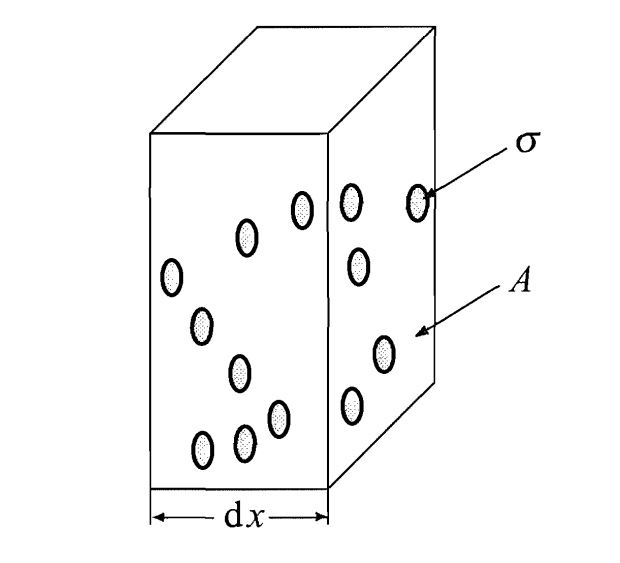
\includegraphics[width=0.4\textwidth]{Images/Stationary-Target-Volume.PNG}\label{fig:f2}}
        \caption{Volume of Stationary Targets.\cite{Plasma}}
    \end{figure}
Cross section ($\sigma$) is defined as the area surrounding a nucleus that would most certainly cause a nuclear reaction if an incident particle passed through this area. It is important to note that this metric is not a physical characteristic, but it is derived from experiment to describe the probability of an interaction. The cross section relates to collision frequency via the mean free path. The flux of incident particles ($\Gamma$) is, by definition the total number of particles crossing Area (A) per unit time, per unit area.
\begin{gather*}d\Gamma=-\sigma * n_1 * \Gamma dx\end{gather*}
With $n_1$ representing the density of target particles and a partial differential equation solution the mean free path ($\lambda$) becomes:
\begin{gather*}\lambda_m = \frac{1}{n_1 * \sigma}\end{gather*}
If the incident particle is moving with a velocity (v) then the corresponding time before having a collision ($\tau_m$) is
\begin{gather*}\tau_m = \frac{\lambda_m}{v}=\frac{1}{n_1 * \sigma * v}\end{gather*}
and the collision frequency ($\nu_m$) is 
\begin{gather*}\nu_m = \frac{1}{\tau_m}=n_1 * \sigma *v\end{gather*}
Transitioning from a small number of nuclear collisions to an industrial size we will need a reaction rate with thermodynamic variable scales. The Hard-sphere reaction rate ($R_{12}$) with 1, the incident particles, and 2, the target is
\begin{gather*}R_{12} = n_1 * n_2 * \sigma * v\end{gather*}
If each collision generates a specific energy ($E_f$) then the power density ($S_f$) can be calculated. $E_f$ can refer to the total energy produced from fusion or the partial energy of the fusions products, alpha particles or neutrons. 
\begin{gather*}S_f = E_f * n_1 * n_2 * \sigma * v\end{gather*}
This previous formulation is a dramatic simplification. To have a more detailed prediction, we must assume that the both Deuterium and Tritium particles are moving with non-uniform velocities. We will consider these velocities to be random. This is accomplished by introducing a distribution function ($f(r,v,t)$) that details both the density and the velocities of the particles. This is in contrast to the previous density function ($n(r,t)$). Firstly we will describe a general equation for macroscopic quantities of interest that include the more detailed density function.
By considering the relative velocity between particles as 
\begin{gather*}v=|v_2-v_1|\end{gather*}
The cross section becomes a function of relative velocity 
\begin{gather*}\sigma=\sigma*(|v_2-v_1|)\end{gather*}
The reaction rate becomes 
\begin{gather*}R_{12}=n_1*n_2 * <\sigma * v>\end{gather*}
The power density becomes
\begin{gather*}S_f=E_fn_1n_2<\sigma v>\end{gather*}
The formulation above assumes that the particles generate a uniform energy from exclusivly short range collisions. It would be realistic to assume that Deuterium is deflected by the electrons orbiting the tritium nuclei.
    \begin{figure}[H]
        \centering
        {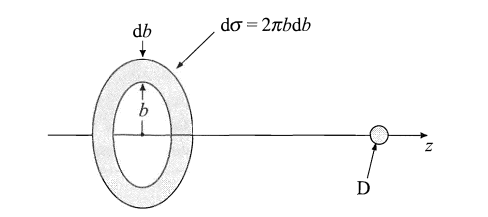
\includegraphics[width=0.4\textwidth]{Images/Differential-CrossSection.PNG}\label{fig:f2}}
        \caption{Differential cross section. \cite{Plasma}}
    \end{figure}
The particles are now dependent on the impact parameter (b), the distance between the moving particle parth and the coulumb interacting source.
\begin{gather*}d\sigma=2*\pi*b*db\end{gather*}
For any macroscopic quantity of interest, including reaction rate and power density, we use $w$:
\begin{gather*}w=2*\pi *\int_{0}^{\infty} {W(v,b)*f_1(v_1)*f_2(v_2)*vb*db*dv_1*dv_2}\end{gather*}
For short-range collisions in nuclear reactors we chose the microscopic quantity of interest (W) to be
\begin{gather*}W=E_f*H(b_0-b)\\b_0^2=\frac{\sigma(v)}{\pi}\end{gather*}
with H representing the Heaviside step function.
Finally, the more detailed distribution functions and their impact on collision prediction. Considering the fact that the long distance coulomb interactions will have a trajectory impact that deters nuclei from colliding the general distribution function for a Deuterium-Tritium reaction is as follows
\begin{gather*}f_j(r,v,t) = n_j * \frac{m_j}{2*\pi*T_j}^\frac{3}{2} * e^\frac{-m_j*\vec{v}^2}{2*T_j}\end{gather*}
$n_j$ denotes particle number density, $T_j$ denotes particle collective temperature, $m_j$ denotes particle mass, v has and x, y, and z spacial coordinate, and the j represents either the fuel source, Deuterium or Tritium. 
\newline
The above variables are thermodynamic in nature and can be measure with precision with the exception of the cross section. We have since assumed that the particles act as billiard balls having a cross section of 
\begin{gather*}\sigma = \pi * d^2\end{gather*}
As with the distribution function, we need to now consider the coulomb's force on the cross section. If a particle is moving fast enough, the Coulomb's force will have negligible effect. "Fast enough" can be formulated by the following
\begin{gather*}
    K_{cm}=\frac{1}{2}*m_r*\vec{v}^2 \geq \frac{e^2}{4*\pi*\epsilon_0 * d} \approx 288 [keV]\\
    m_r = \frac{m_D * m_T}{m_D + m_T}
\end{gather*}
$m_r$ denotes the reduced mass, $m_D$ and $m_T$ denote the mass of Deuterium and Tritium, v vector denotes the velocity of the incident particle with the other particle being stationary, $e_0$ denotes vacuum permittivity, d denotes the diameter of the particles (assuming they are identical), and $K_{cm}$ denotes the center of mass kinetic energy. Any particle that has less than $K_{cm}$ will not have nuclear fusion occur. 
\newline
$K_{cm}$ of 288 [keV] is much larger than we see in actual experiments. Quantum mechanical effects such as Quantum Tunneling, Resonance, and high-speed decay create unpredictable conditions. 
    \begin{figure}[H]
        \centering
        {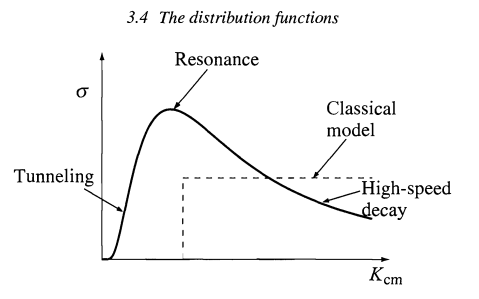
\includegraphics[width=0.4\textwidth]{Images/Quantum-CrossSection.PNG}\label{fig:f2}}
        \caption{Quantum cross section. \cite{Plasma}}
    \end{figure}
In practice, the cross section is determined experimentally.
    \begin{figure}[H]
        \centering
        {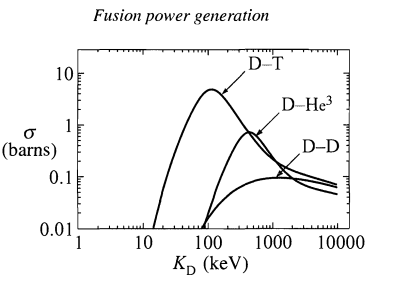
\includegraphics[width=0.4\textwidth]{Images/FuelComp-CrossSection.PNG}\label{fig:f1}}
        \caption{Fuel cross section comparison. \cite{Plasma}}
    \end{figure}
This overview of the fusion history and collision requirements provides and great base for comparing the challenges that face us today. In comparison to fusion, the cross section of the larger fission reactor fuels is certainly a large advantage. If the fuels could be heated to a dramatically higher temperature then the collision frequency would also increase. As we increase the density, the fuel becomes increasingly unstable. In conclusion, the core issues facing the development of fusion energy are fuel choice, heating and current drive, subsequently transport, and macroscopic equilibrium and stability. By comparing the currently investigated methods we can gain a better understanding of how they each perform.
\newline
This mathematical formulation can be attributed to reference \cite{Plasma}


\section{Global Fusion Industry in 2023}
The "Wrights Brothers" moment from Livermore National Laboratory in 2022 sparked interest in the energy sector and from nations world wide to invest time, energy, and resources to making a fusion driven electrical grid a reality. In 1 year, nearly \$1.4 billion was invested, publicly and privately, across 12 countries. This massive investment is mostly intended to use fusion technology for electricity generation and space propulsion. The following image details the distribution of approaches from those companies and government laboratories:
    \begin{figure}[H]
        \centering
        {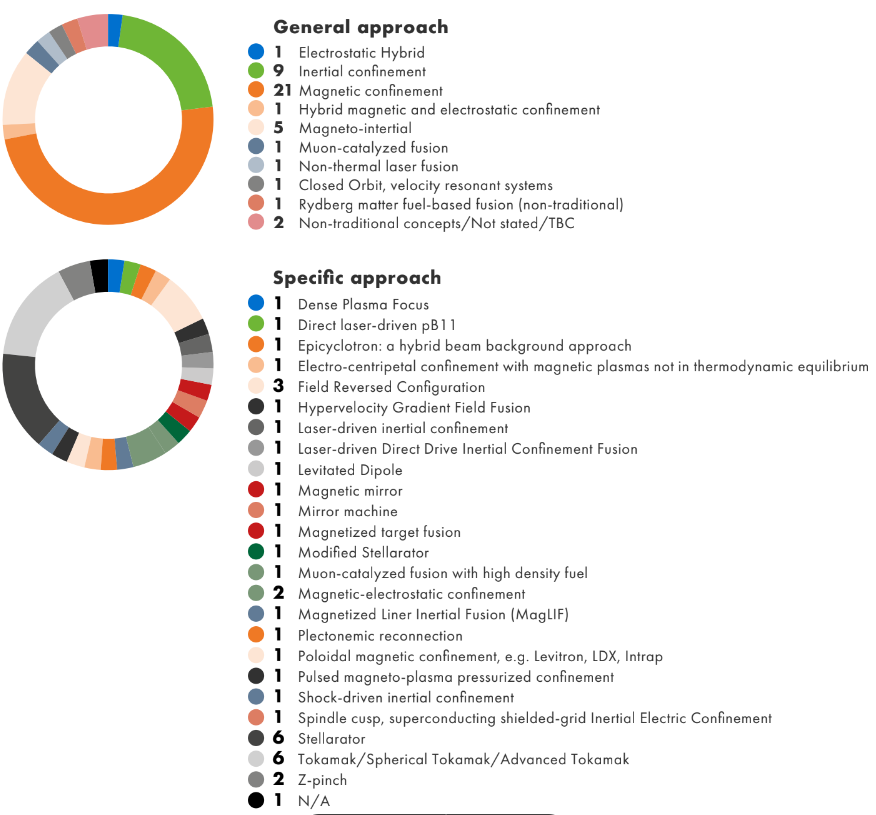
\includegraphics[width=1\textwidth]{Images/Approach2.PNG}\label{fig:f2}}
        \caption{Fusion Approach Distribution. \cite{FIA23}}
    \end{figure}

\subsection{Basic Beginnings}
In march of 1951, Ronald Richter, an Austian-born Argentinian immigrant, had convinced the authorities to build a large secret fusion lab on the remote island, Isla Huemul. In the concrete surrounded laboratory in the Argentinian wilderness they reported a "net positive result" for the first time. This laboratory fed hydrogen into an electric arc and recorded the resulting temperature. The temperature recorded was above which is required for nuclear reactions to occur, but did not intend to measure any fusion byproducts. This discovery nearly led the Argentinian president, Juan Peron, to invade the Falkland Islands with the belief that they would be the first to exploit atomic energy. Reference \cite{6}. The eventual next steps were to confine this plasma, which was much more difficult and time consuming than Juan Peron assumed.
%Peron Needs Accent
%https://en.wikipedia.org/wiki/Juan_Per%C3%B3n
    \begin{figure}[H]
        \centering
        \subfloat[Perhapsatron]{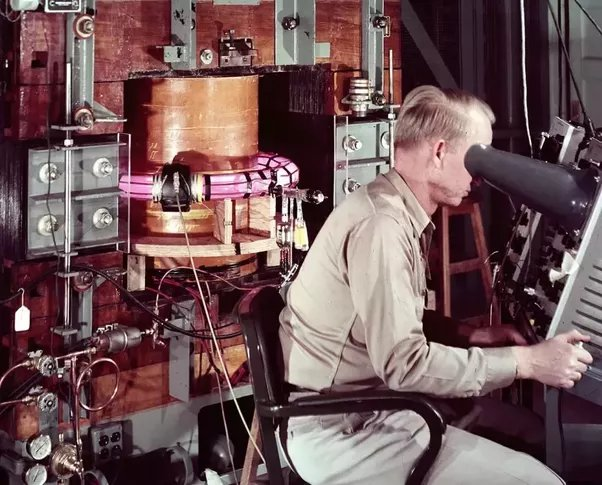
\includegraphics[width=0.3\textwidth]{Images/Perhapsatron.jpg}\label{fig:f1}}
        \hfill
        \subfloat[Huemul Island]{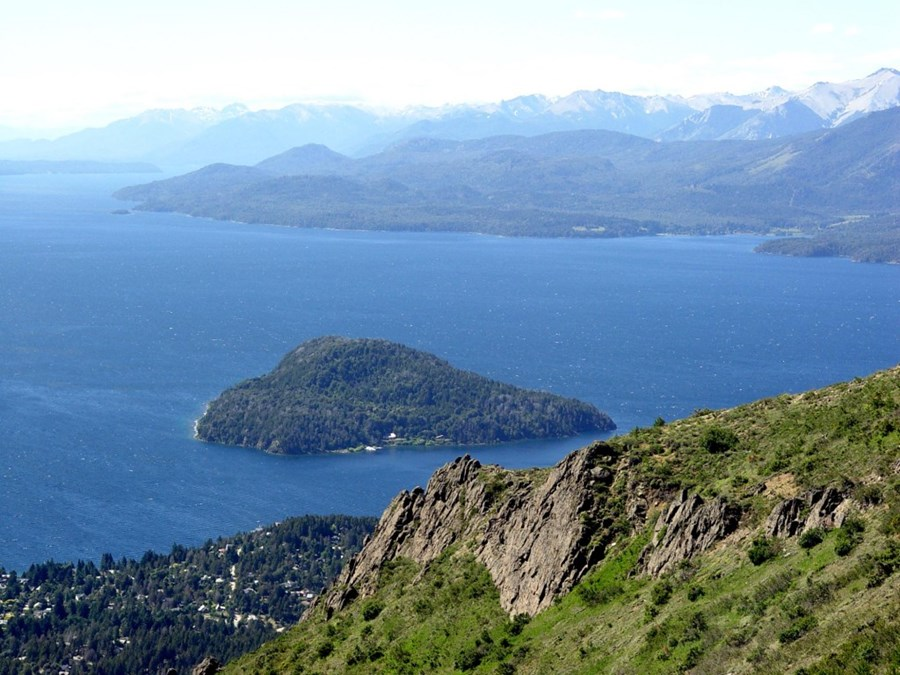
\includegraphics[width=0.3\textwidth]{Images/HuemulIsle.jpg}\label{fig:f2}}
        \hfill
        \subfloat[Huemul Building]{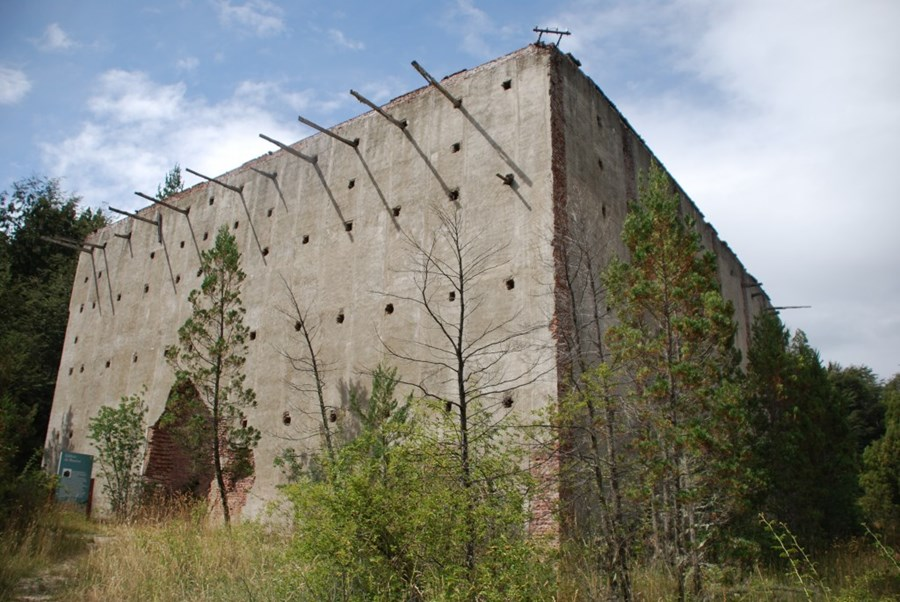
\includegraphics[width=0.3\textwidth]{Images/HuemulBuilding.jpg}\label{fig:f3}}
    \end{figure}

\subsection{Magnetic Confinment Fusion (MCF)}
Z-Pinch or Zeta-Pinch is a method which constrains and compresses a plasma by providing electric current orthogonal to the direction of the plasma. The electric current induces a magnetic field within the plasma which causes its confinement. After the discovery made by Ronald Richter most of the designs constricted plasma along the inside of a toroid. This quickly lead to fluid related instabilities where the dense plasma at the center of the toroid interacted with the lighter plasma at the edges of the toroid, leading to Raleigh-Taylor and Richtmyer-Meshkov instabilities. 
\newline
    \begin{figure}[H]
        \centering
        \subfloat[Richtmyer-Meshkov Instability]{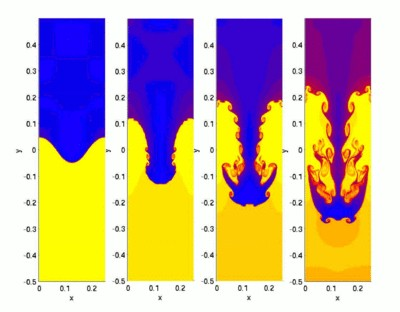
\includegraphics[width=0.4\textwidth]{Images/RM Instability.jpg}\label{fig:f1}}
        \hfill
        \subfloat[Toroidal Coordinates. Polidal ($\theta$-Red Arrow), and Toroidal ($\varphi$-Blue Arrow. \cite{TorCoor}]{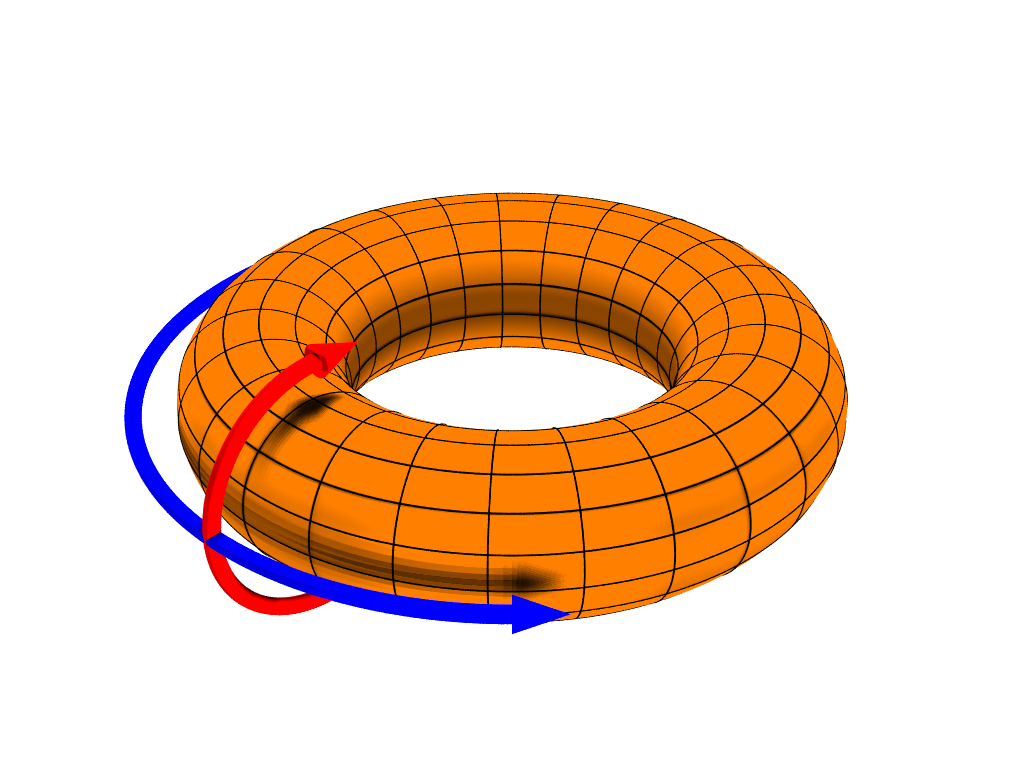
\includegraphics[width=0.4\textwidth]{Images/Toroidal_coord.png}\label{fig:f2}}
    \end{figure}
The current was originally just poloidal, then a toroidal current was introduced. This made progress but did not solve the fluid instability. The ZETA project began operation in 1957 in the UK by adding magnets poloidally to increase the stability of confinement. While previous experiments rarely lasted longer than a few microseconds, the ZETA project passed the millisecond mark. In the late 1960's USSR built the Tokomak, which similarly provided electric current to the plasma and further confined the plasma with poloidal exterior magnets. The important difference that led to the Tokamak-3 (T-3) producing the first verifiable nuclear fusion reactions was the strength and shape of the magnetic field, the proportions of the axial symmetric torus, and the current injected into the plasma. Reaching 1 [keV], the T-3 successfully produced neutrons that matched theories as being produced by fusion. The Tokamak style of fusion reactor became, and still is, the most heavily researched reactor in the world. The exterior magnetic components induced a helix motion within the plasma field so the Stellerators were design with magnets that matched the motion to create greater stability. Changing the geometric shape, the spherical tokamak improved stability parameters and is the most successful fusion reactor to date. 
These design changes were all to benifit stability. 
%Go into detail about current affairs of tokamaks
%\cite{8}

\subsection{Inertial Confinement Fusion (ICF)}
The first uses of ICF were the Hydrogen Bombs. In a single casing there was a fission explosion that gave off X-Rays which in turn cause the fusion fuel to compress and heat causing it to explode. ICF devices that rely exclusively on fusion reactions depend on other methods to heat and compress the atoms. Laser based ICF began in the early 1970's, most notably with the Shiva and Nova lasers built at Livermore National Laboratory. The two laser had less than satisfactory fusion yields because of premature heating of the dense plasma and laser coupling with hot electrons. Progress from these lasers led to the construction of the National Ignition Facility which sets record for the first to achieve scientific break-even on December 5 of 2022. 

\begin{comment}
\subsection{Summary of Fusion Methods and Experiments}
\begin{table}
    \centering
    \begin{tabular}{cccclll}
         Experiment&  Company (Nation)&  Confinement Type& Processes Category &Years &Q Plasma Value&Website\\
         International Thermonuclear Experimental Reactor (ITER)&  (International)&  Magnetic &  Tokamak&2013-2025 &10&https://www.iter.org/\\
 Demonstration Power Plant (DEMO)& (International)& Magnetic& Tokamak& 2017-2048& 25&https://euro-fusion.org/programme/demo/\\
 (PROTO)& (International)& Magnetic& Tokamak& 2050-Future& N/A&\\
 STOR-M& Fusion Energy Base (Canada)& Magnetic& Tokamak& 1987-Present& &http://plasma.usask.ca/fusion/storm.php\\
 Acator C-Mod& MIT (USA)& Magnetic& Tokamak& 1993-2016& &https://www.psfc.mit.edu/research/topics/alcator-c-mod-tokamak\\
 SPARC& Commonwealth (USA)& Magnetic& Tokamak& & 2&https://cfs.energy/technology/sparc\\
 DIII-D& General Atomics (USA)& Magnetic& Tokamak& 1980-& &https://www.ga.com/magnetic-fusion/diii-d\\
 Enourmous Toroidal Plasma Device (ETPD)& University of California (USA)& Magnetic& Tokamak& 1999-2006, amd 2009-& &\\
 Lithium Tokamak Experiment (LTX)& Princeton University (USA)& Magnetic& Tokamak (Spherical)& 2008-Present& &https://www.pppl.gov/research/projects/lithium-tokamak-experiment\\
 Princeton Large Torus (PLT)& Princeton University (USA)& Magnetic& Tokamak (Spherical)& 1975-1986& &\\
 Tokamak Fusion Test Reactor (TFTR)& Princeton University (USA)& Magnetic& Tokamak (Spherical)& 1982-1997& &\\
 National Spherical Torus Experiment (NSTX)& Princeton University (USA)& Magnetic& Tokamak (Spherical)& 1999-Present& &\\
 Pegasus& University of Wisconsin (USA)& Magnetic& Tokamak (Spherical)& Upgraded in 2019& &\\
 & & & & & &\\
 & & & & & &\\
 & & & & & &\\
 & & & & & &\\
    \end{tabular}
    \caption{Caption}
    \label{tab:my_label}
\end{table}
\end{comment}

\section{Catalyst}
Magnetic confinement, gravitational confinement, inertial confinement, electrostatic confinement, and acoustic cavitation are example of processes developed over the past 70 years to overcome the high temperature required for fusion to occur, the instability of highly magnetized plasma's, and the challenge of easily collecting the energetic products. With the current methods this is mostly a engineering, economical, and political challenge. Large experimental nuclear reactors are difficult to fund without massive government contracts or passionate and wealthy donors. The power of magnets and lasers are ever progressing material challenges whose applications span a wide variety of fields. The most ideal nuclear reactor is the one that produced no radioactive waste, is self-sustained, requires very little startup energy, and is as small as possible. In reality, the first nuclear reactors to produce energy for the worlds use will likely be large production stations with sufficient safety measures and electrical distribution infrastructure. We could make progress toward the ideal scenario if the requirements for nuclear fusion could be reduced. In nature, i.e. the fusion within the sun, all reactions take the easiest and least energetic path possible. This axiom was revolutionary in chemistry, and the development of Catalysts were the forefront of bringing down the energy requirements of reactions. 
\newline
This could be the case for fusion reactions as well. The scheme of additing $\mu$ mesons to the deuterium atom in place of electrons was first introduced by a team at the University of California's Radiation Laboratory [\cite{MuonCat}]. It was discovered somewhat by accident when an experiment involving the stopping of negative K mesons into a bubble chamber produced an interesting new reaction. The experiment showed more $\mu$ and less K mesons than expected and produced more energy than expected. They predicted that the results of their test were that the $\mu$ shrunk the cross section of the hydrogen ion leading to more frequent nuclear reactions. Even in this initial experiment they noticed some energy was being siphoned off. It was later determined that the $\mu$ "stick" to the fusion by products.
    \begin{figure} [H]
        \centering
        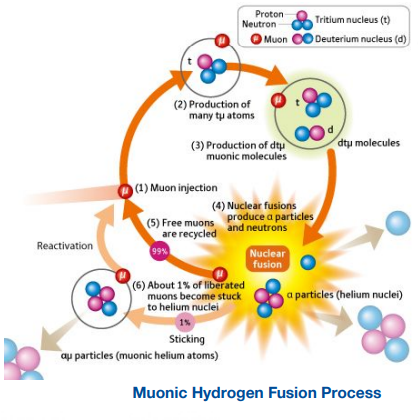
\includegraphics[width=0.5\linewidth]{Images/Muonic Hydrogen Fusion Process.png}
        \caption{Muonic Hydrogen Fusion Process \cite{HighYieldMuCat}}
        \label{fig:enter-label}
    \end{figure}
The In-flight Muon Catalyzed Fusion (IFMCF) muonic atom-nucleus collision cross section was calculated with improved precision to be 2000 [barns] at 1.4 [keV] \cite{MuCatFut}. For comparison, regular deuterium-tritium fusion cross-section was evaluated to be $1.171*10^-6$ [Barns] at 1 [keV] \cite{FuCross}. In the original "cold" Muon Catalyzed fusion context, the target has to be highly dense and cold in a ice or liquid hydrogen form to attain fusion reactions. The technical challenges of keeping a hydrogen isotope as an ice or liquid has been dismissed as unrealistic because of the "sticking" problem. The $\mu$ mesons would stick to the $\alpha$ particles after the nuclear reaction at a 0.3\% rate, causing a muon cycle of only about 100 during its short lifetime. By skipping the $\mu$ transfer and molecular formation process and attain nuclear fusion in flight a cycle of nearly 1000 can take place \cite{MuCatFut}. This method could achieve Q>1 with existing technologies. The fusion takes place in the shock wave of a supersonic flow and there is no tight energy balance, as Magnetic Fusion requires, or homogeneous implosion, as Inertial Fusion requires.
\newline
Another proposed solution to the $\mu$ "sticking" problem is replacing the Deuterium-Tritium-$\mu$ (dt$\mu$) molecule with a muonic Lithium hydride ($LiH^+$) (Reference \cite{wu2022investigating}). According to \cite{PhysRev.106.330}, the alpha sticking problem strongly depends on the velocity of the outgoing alpha particle. The fusion reaction $Li+p\rightarrow 2\alpha$ carries more momentum than the typical Deuterium-Tritium reaction $d+t\rightarrow\alpha+n$. Additionally the Lithium has more electric charges which may help the muon be recaptured. 
\newline
Muons are costly and difficult to produce because they require high energy accelerators. Additionally, muons have a very short life span; therefore, the muons would need to be created in line with the fusion producing mechanisms. 
\newline 
While muons are the only know particle additive that would effectively catalyze nuclear fusion there are groups considering alternatives. As has been discussed the Coulomb barrier is among the largest hurtle in nuclear fusion, but it may be possible to fuse specific nuclei by controlling electron wave functions in intense laser fields. The circularly polarized chiral laser field can effectively squeeze the electrons wave functions, lowering the coulomb barrier. The Sommerfeld parameter ($\eta$) at a given center of mass kinetic energy ($K_{cm}$):
\begin{gather*}
    \nu(K_{cm})=\sqrt{\frac{2K_{cm}}{\mu}}\\
    \mu=\frac{M_1M_2}{M_1+M_2}
    \eta(K_{cm})=\frac{Z_1Z_2e^2}{\nu(K_{cm})}\\
    \sigma(K_{cm})=\frac{S(K_{cm})}{K_{cm}}e^{-2\pi\eta(K_{cm})}\\
    U(r)=\frac{Z_1Z_2e^2}{r_c}\\
\end{gather*}
where $Z_1$, $Z_2$, $M_1$, and $M_2$ are the electrical charge and mass, respectively, of the colliding nuclei, $S(K_{cm})$ is the "astrophysical S-factor" that accounts for nuclear interactions, $\nu(K_{cm}$ is the relative velocity. To properly account for the Coulomb screening:
\begin{gather*}
    U(r)=\frac{Z_1Z_2e^2}{r_c}e^{-\frac{r_c}{r_D}}\\
    U_0=\frac{Z_1Z_2e^2}{r_D}\\
    R_s(K_{cm})\equiv\frac{e^{-2 \pi \eta (K_{cm} + U_0})}{e^{-2 \pi \eta (K_{cm})}}
\end{gather*}
where $r_D$ is the screening radius (ideally the Bohr radius = 
$r_B=(M_e c \alpha)^-1=0.53 \r{A}$ and $U_0$ is the difference between the energy of the compound atom and the sum of the energies of atoms before fusion (For D-H $U_0\simeq 24$ [eV]. If $Z_2>>Z_1$ then we can neglect the coulomb screening around nucleus 1. 
\begin{gather*}
    R_s(K_{cm})\simeq e^{\pi \eta (K_{cm}) \frac{U_0}{K_cm}}\\
    K_cm >> U_0
\end{gather*}
This provides an exponential enhancement to the fusion cross section at low energies confined by experiment \cite{PhysRev.106.330}.
For circularly polarized laser fields the electron distribution becomes ring-like. The radius of the ring is equal to classical excursion parameter ($r_c$) 
\begin{gather*}
    r_c=\frac{e k_{cm}}{m_e \omega^2}
\end{gather*}
which corresponds to the circular motion of the electron that is phase locked with the electric field of the laser.
This method has the possibility of reducing the Coulomb screening radius by a factor of tens or hundreds. The reduction required to fuse the components of water molecules is merely 5.  
 %Function of adding catalyist
 %Proposals
 %What is the few body Schrodinger equation
 %What is the Gaussian expansion method (GEM)
%\section{Heating and current drive ch 15}
%ore issues facing the development of fusion energy: Macroscopic equilibrium and stability, transport, and heating and current drive.
%Frontier of plasma physics - alpha particle plasma physics
%\section{heating and current progress}



\newpage
\printbibliography
\end{document}
